\subsection{Explicit Prompting Improves Initial Quality, But Still Degrades}
\label{sec:prompt-strategy}
We next evaluate whether prompt-side modifications can mitigate the degradation induced by iteration. Two prompts are tested against the \justsolve{}~ baseline. \antislop{} (\autoref{lst:anti-slop-prompt}) enumerates verbosity and over-engineering patterns the agent should avoid. \planfirst{} (\autoref{lst:plan-first-prompt}) requires the agent to produce a written plan before generating code.

\begin{figure}[t]
    \centering
    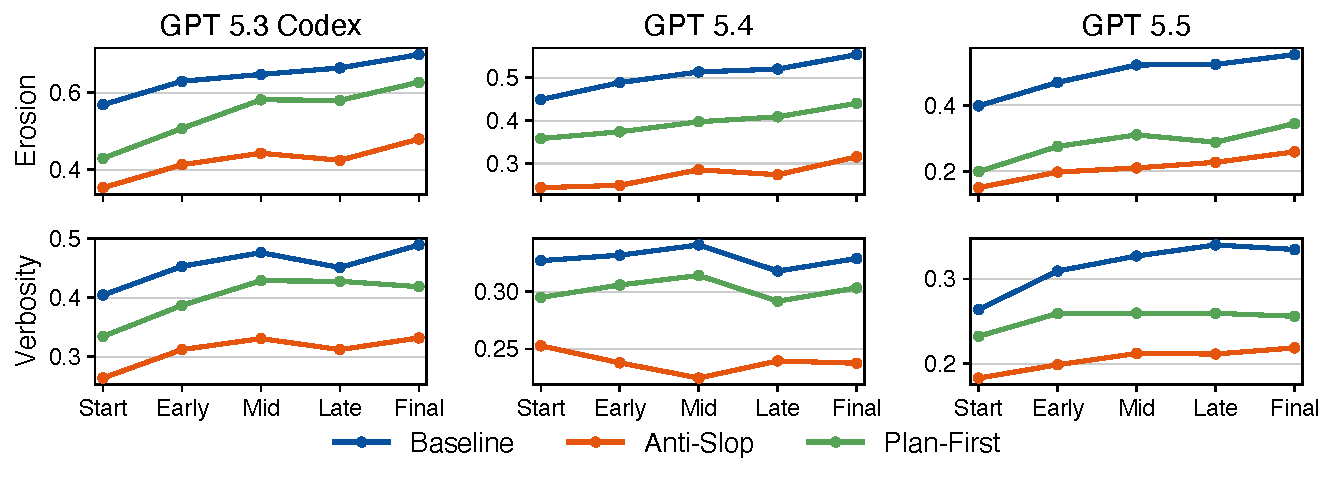
\includegraphics[width=\textwidth]{figures/prompt_strategy_trajectories.pdf}
    \caption{\textbf{Prompting can improve initial quality, but does not remove the iterative issues.} Mean structural erosion (top) and verbosity (bottom) at each progress bin, per model.}
    \label{fig:prompt-strategy-trajectories}
\end{figure}

\definecolor{good}{HTML}{1B7837}
\definecolor{bad}{HTML}{B2182B}
\begin{table}[t]
    \centering
    \caption{Raw values per prompt with the lift over \justsolve{} in parentheses. \textcolor{good}{Green} means improvements while \textcolor{bad}{red} indicates regressions.}
    \label{tab:prompt-strategy-lift}
    \footnotesize
    \setlength{\tabcolsep}{5pt}
    \begin{tabular}{llcccccc}
        \toprule
        Model & Prompt & Strict & Iso. & Core & Erosion & Verbosity & Cost \\
        \midrule
        \multirow{3}{*}{GPT 5.3 Codex} & Just-Solve & 11.2 & 26.0 & 60.7 & 0.64 & 0.46 & 0.66 \\
         & Anti-Slop & 11.2 (+0.0) & 23.5 (\textcolor{bad}{-2.6}) & 57.1 (\textcolor{bad}{-3.6}) & 0.42 (\textcolor{good}{-0.22}) & 0.31 (\textcolor{good}{-0.15}) & 0.73 (\textcolor{bad}{+0.07}) \\
         & Plan-First & 8.2 (\textcolor{bad}{-3.1}) & 21.4 (\textcolor{bad}{-4.6}) & 62.2 (\textcolor{good}{+1.5}) & 0.55 (\textcolor{good}{-0.10}) & 0.40 (\textcolor{good}{-0.06}) & 0.68 (\textcolor{bad}{+0.02}) \\
        \midrule
        \multirow{3}{*}{GPT 5.4} & Just-Solve & 10.7 & 23.5 & 62.8 & 0.51 & 0.33 & 0.72 \\
         & Anti-Slop & 9.2 (\textcolor{bad}{-1.5}) & 25.5 (\textcolor{good}{+2.0}) & 61.2 (\textcolor{bad}{-1.5}) & 0.28 (\textcolor{good}{-0.23}) & 0.24 (\textcolor{good}{-0.09}) & 0.90 (\textcolor{bad}{+0.18}) \\
         & Plan-First & 9.7 (\textcolor{bad}{-1.0}) & 25.0 (\textcolor{good}{+1.5}) & 63.3 (\textcolor{good}{+0.5}) & 0.39 (\textcolor{good}{-0.11}) & 0.30 (\textcolor{good}{-0.02}) & 0.83 (\textcolor{bad}{+0.11}) \\
        \midrule
        \multirow{3}{*}{GPT 5.5} & Just-Solve & 14.8 & 28.1 & 66.8 & 0.49 & 0.32 & 1.51 \\
         & Anti-Slop & 9.2 (\textcolor{bad}{-5.6}) & 24.0 (\textcolor{bad}{-4.1}) & 63.3 (\textcolor{bad}{-3.6}) & 0.21 (\textcolor{good}{-0.28}) & 0.21 (\textcolor{good}{-0.11}) & 1.68 (\textcolor{bad}{+0.17}) \\
         & Plan-First & 8.2 (\textcolor{bad}{-6.6}) & 24.0 (\textcolor{bad}{-4.1}) & 67.3 (\textcolor{good}{+0.5}) & 0.29 (\textcolor{good}{-0.21}) & 0.25 (\textcolor{good}{-0.06}) & 1.61 (\textcolor{bad}{+0.11}) \\
        \bottomrule
    \end{tabular}
\end{table}



\autoref{fig:prompt-strategy-trajectories} highlights that the magnitudes of structural erosion and verbosity are significantly lowered by prompt strategies. Under \antislop{}, verbosity is lower than baseline by \psGptFiveFourAntiSlopVerbPctRed\% on GPT~5.4, \psGptFiveFiveAntiSlopVerbPctRed\% on GPT~5.5, and \psCodexAntiSlopVerbPctRed\% on GPT~5.3~Codex. Erosion is lower by \psGptFiveFourAntiSlopEroPctRed\%, \psGptFiveFiveAntiSlopEroPctRed\%, and \psCodexAntiSlopEroPctRed\% respectively. Only with GPT 5.4 do we observe that quality \emph{improves} from start to end with the \antislop{} prompt.

This improved quality comes with some trade-offs, as highlighted in \autoref{tab:prompt-strategy-lift}. Across models, the base \justsolve~prompt has the best strict performance with an average drop of \psLiftStrictDropAntiSlop~pp for \antislop~and \psLiftStrictDropPlanFirst~pp for \planfirst. Core pass rate improves by 0.8~pp for \planfirst. Both prompts raise the cost per checkpoint by \psLiftCostIncreasePct\% on average. \textbf{Overall, prompting strategies trade capabilities for better initial quality, with little impact on the iterative degradation.}